\documentclass[1p]{elsarticle_modified}
%\bibliographystyle{elsarticle-num}

%\usepackage[colorlinks]{hyperref}
%\usepackage{abbrmath_seonhwa} %\Abb, \Ascr, \Acal ,\Abf, \Afrak
\usepackage{amsfonts}
\usepackage{amssymb}
\usepackage{amsmath}
\usepackage{amsthm}
\usepackage{scalefnt}
\usepackage{amsbsy}
\usepackage{kotex}
\usepackage{caption}
\usepackage{subfig}
\usepackage{color}
\usepackage{graphicx}
\usepackage{xcolor} %% white, black, red, green, blue, cyan, magenta, yellow
\usepackage{float}
\usepackage{setspace}
\usepackage{hyperref}

\usepackage{tikz}
\usetikzlibrary{arrows}

\usepackage{multirow}
\usepackage{array} % fixed length table
\usepackage{hhline}

%%%%%%%%%%%%%%%%%%%%%
\makeatletter
\renewcommand*\env@matrix[1][\arraystretch]{%
	\edef\arraystretch{#1}%
	\hskip -\arraycolsep
	\let\@ifnextchar\new@ifnextchar
	\array{*\c@MaxMatrixCols c}}
\makeatother %https://tex.stackexchange.com/questions/14071/how-can-i-increase-the-line-spacing-in-a-matrix
%%%%%%%%%%%%%%%

\usepackage[normalem]{ulem}

\newcommand{\msout}[1]{\ifmmode\text{\sout{\ensuremath{#1}}}\else\sout{#1}\fi}
%SOURCE: \msout is \stkout macro in https://tex.stackexchange.com/questions/20609/strikeout-in-math-mode

\newcommand{\cancel}[1]{
	\ifmmode
	{\color{red}\msout{#1}}
	\else
	{\color{red}\sout{#1}}
	\fi
}

\newcommand{\add}[1]{
	{\color{blue}\uwave{#1}}
}

\newcommand{\replace}[2]{
	\ifmmode
	{\color{red}\msout{#1}}{\color{blue}\uwave{#2}}
	\else
	{\color{red}\sout{#1}}{\color{blue}\uwave{#2}}
	\fi
}

\newcommand{\Sol}{\mathcal{S}} %segment
\newcommand{\D}{D} %diagram
\newcommand{\A}{\mathcal{A}} %arc


%%%%%%%%%%%%%%%%%%%%%%%%%%%%%5 test

\def\sl{\operatorname{\textup{SL}}(2,\Cbb)}
\def\psl{\operatorname{\textup{PSL}}(2,\Cbb)}
\def\quan{\mkern 1mu \triangleright \mkern 1mu}

\theoremstyle{definition}
\newtheorem{thm}{Theorem}[section]
\newtheorem{prop}[thm]{Proposition}
\newtheorem{lem}[thm]{Lemma}
\newtheorem{ques}[thm]{Question}
\newtheorem{cor}[thm]{Corollary}
\newtheorem{defn}[thm]{Definition}
\newtheorem{exam}[thm]{Example}
\newtheorem{rmk}[thm]{Remark}
\newtheorem{alg}[thm]{Algorithm}

\newcommand{\I}{\sqrt{-1}}
\begin{document}

%\begin{frontmatter}
%
%\title{Boundary parabolic representations of knots up to 8 crossings}
%
%%% Group authors per affiliation:
%\author{Yunhi Cho} 
%\address{Department of Mathematics, University of Seoul, Seoul, Korea}
%\ead{yhcho@uos.ac.kr}
%
%
%\author{Seonhwa Kim} %\fnref{s_kim}}
%\address{Center for Geometry and Physics, Institute for Basic Science, Pohang, 37673, Korea}
%\ead{ryeona17@ibs.re.kr}
%
%\author{Hyuk Kim}
%\address{Department of Mathematical Sciences, Seoul National University, Seoul 08826, Korea}
%\ead{hyukkim@snu.ac.kr}
%
%\author{Seokbeom Yoon}
%\address{Department of Mathematical Sciences, Seoul National University, Seoul, 08826,  Korea}
%\ead{sbyoon15@snu.ac.kr}
%
%\begin{abstract}
%We find all boundary parabolic representation of knots up to 8 crossings.
%
%\end{abstract}
%\begin{keyword}
%    \MSC[2010] 57M25 
%\end{keyword}
%
%\end{frontmatter}

%\linenumbers
%\tableofcontents
%
\newcommand\colored[1]{\textcolor{white}{\rule[-0.35ex]{0.8em}{1.4ex}}\kern-0.8em\color{red} #1}%
%\newcommand\colored[1]{\textcolor{white}{ #1}\kern-2.17ex	\textcolor{white}{ #1}\kern-1.81ex	\textcolor{white}{ #1}\kern-2.15ex\color{red}#1	}

{\Large $\underline{12a_{0661}~(K12a_{0661})}$}

\setlength{\tabcolsep}{10pt}
\renewcommand{\arraystretch}{1.6}
\vspace{1cm}\begin{tabular}{m{100pt}>{\centering\arraybackslash}m{274pt}}
\multirow{5}{120pt}{
	\centering
	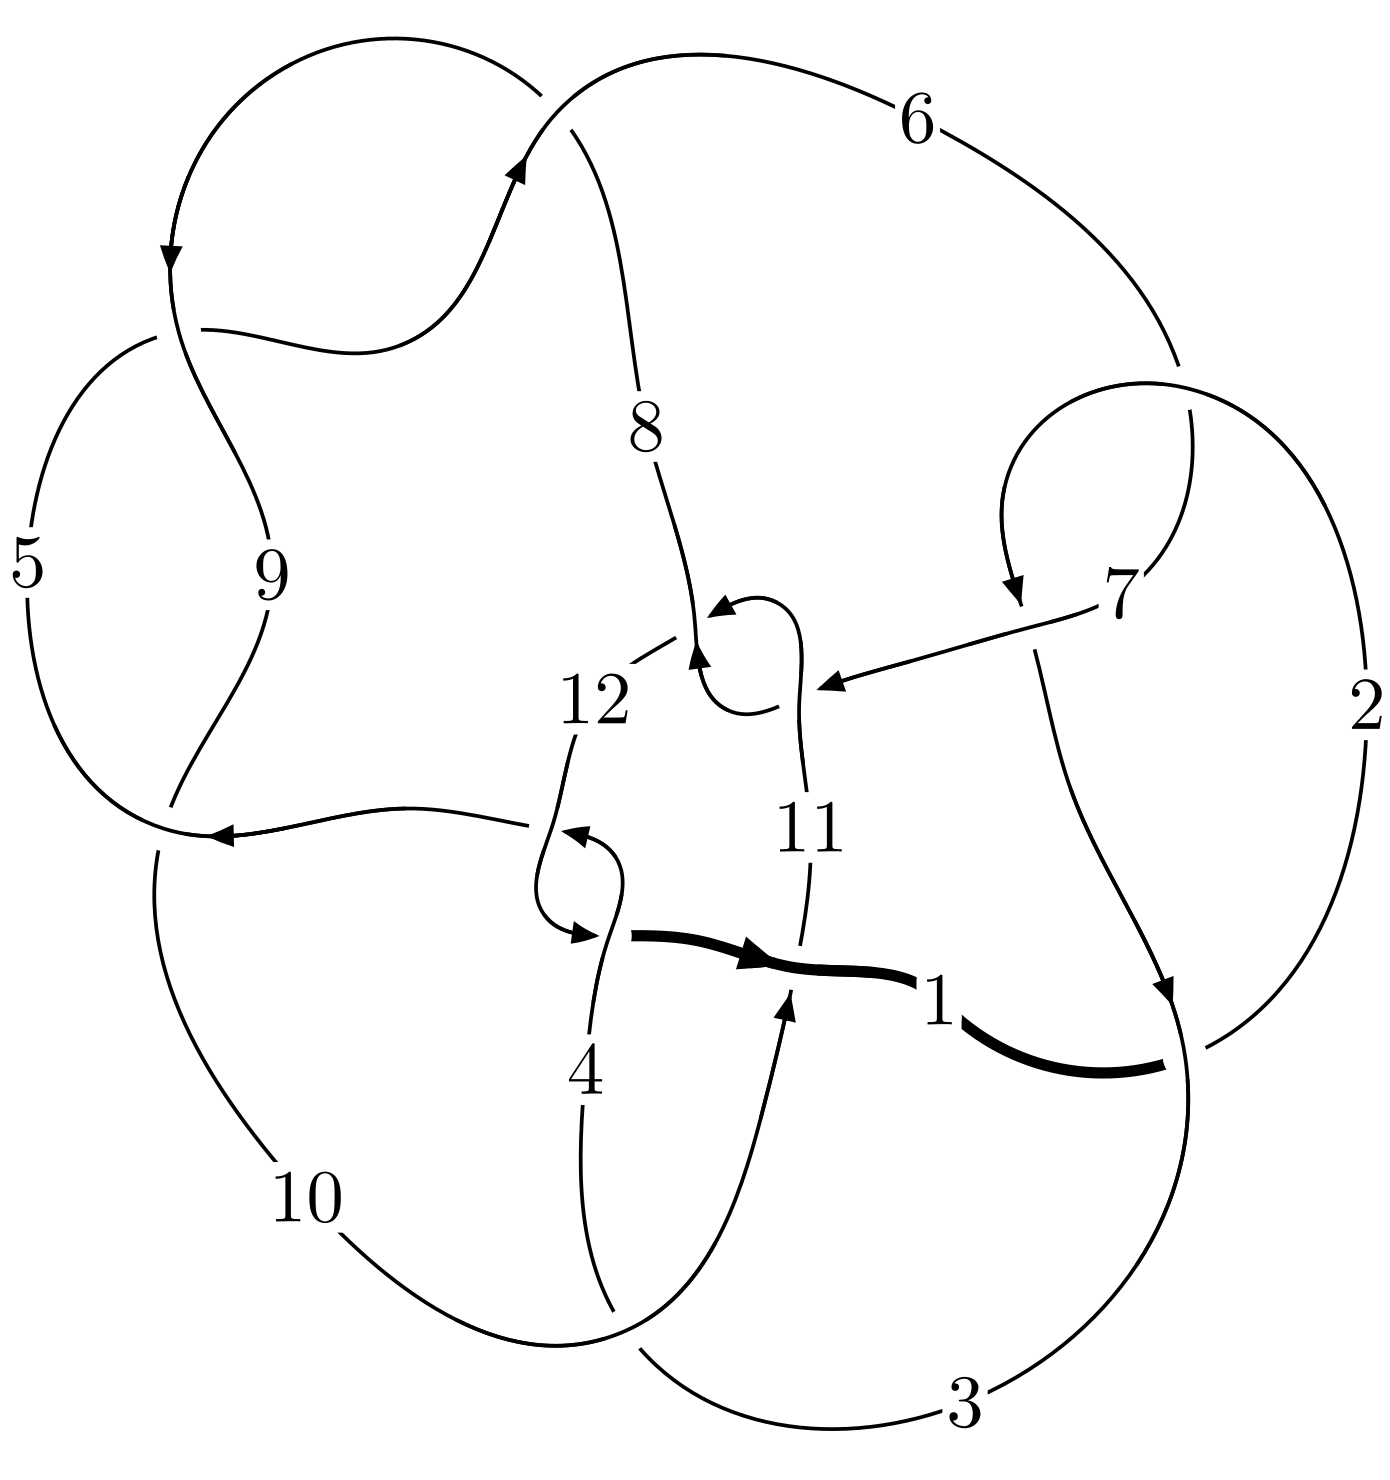
\includegraphics[width=112pt]{../../../GIT/diagram.site/Diagrams/png/1462_12a_0661.png}\\
\ \ \ A knot diagram\footnotemark}&
\allowdisplaybreaks
\textbf{Linearized knot diagam} \\
\cline{2-2}
 &
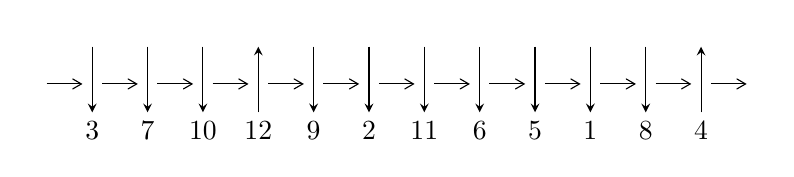
\begin{tikzpicture}[x=20pt, y=17pt]
	% nodes
	\node (C0) at (0, 0) {};
	\node (C1) at (1, 0) {};
	\node (C1U) at (1, +1) {};
	\node (C1D) at (1, -1) {3};

	\node (C2) at (2, 0) {};
	\node (C2U) at (2, +1) {};
	\node (C2D) at (2, -1) {7};

	\node (C3) at (3, 0) {};
	\node (C3U) at (3, +1) {};
	\node (C3D) at (3, -1) {10};

	\node (C4) at (4, 0) {};
	\node (C4U) at (4, +1) {};
	\node (C4D) at (4, -1) {12};

	\node (C5) at (5, 0) {};
	\node (C5U) at (5, +1) {};
	\node (C5D) at (5, -1) {9};

	\node (C6) at (6, 0) {};
	\node (C6U) at (6, +1) {};
	\node (C6D) at (6, -1) {2};

	\node (C7) at (7, 0) {};
	\node (C7U) at (7, +1) {};
	\node (C7D) at (7, -1) {11};

	\node (C8) at (8, 0) {};
	\node (C8U) at (8, +1) {};
	\node (C8D) at (8, -1) {6};

	\node (C9) at (9, 0) {};
	\node (C9U) at (9, +1) {};
	\node (C9D) at (9, -1) {5};

	\node (C10) at (10, 0) {};
	\node (C10U) at (10, +1) {};
	\node (C10D) at (10, -1) {1};

	\node (C11) at (11, 0) {};
	\node (C11U) at (11, +1) {};
	\node (C11D) at (11, -1) {8};

	\node (C12) at (12, 0) {};
	\node (C12U) at (12, +1) {};
	\node (C12D) at (12, -1) {4};
	\node (C13) at (13, 0) {};

	% arrows
	\draw[->,>={angle 60}]
	(C0) edge (C1) (C1) edge (C2) (C2) edge (C3) (C3) edge (C4) (C4) edge (C5) (C5) edge (C6) (C6) edge (C7) (C7) edge (C8) (C8) edge (C9) (C9) edge (C10) (C10) edge (C11) (C11) edge (C12) (C12) edge (C13) ;	\draw[->,>=stealth]
	(C1U) edge (C1D) (C2U) edge (C2D) (C3U) edge (C3D) (C4D) edge (C4U) (C5U) edge (C5D) (C6U) edge (C6D) (C7U) edge (C7D) (C8U) edge (C8D) (C9U) edge (C9D) (C10U) edge (C10D) (C11U) edge (C11D) (C12D) edge (C12U) ;
	\end{tikzpicture} \\
\hhline{~~} \\& 
\textbf{Solving Sequence} \\ \cline{2-2} 
 &
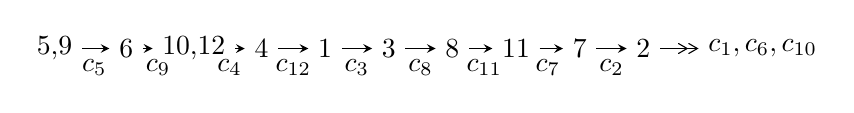
\begin{tikzpicture}[x=23pt, y=7pt]
	% node
	\node (A0) at (-1/8, 0) {5,9};
	\node (A1) at (1, 0) {6};
	\node (A2) at (33/16, 0) {10,12};
	\node (A3) at (25/8, 0) {4};
	\node (A4) at (33/8, 0) {1};
	\node (A5) at (41/8, 0) {3};
	\node (A6) at (49/8, 0) {8};
	\node (A7) at (57/8, 0) {11};
	\node (A8) at (65/8, 0) {7};
	\node (A9) at (73/8, 0) {2};
	\node (C1) at (1/2, -1) {$c_{5}$};
	\node (C2) at (3/2, -1) {$c_{9}$};
	\node (C3) at (21/8, -1) {$c_{4}$};
	\node (C4) at (29/8, -1) {$c_{12}$};
	\node (C5) at (37/8, -1) {$c_{3}$};
	\node (C6) at (45/8, -1) {$c_{8}$};
	\node (C7) at (53/8, -1) {$c_{11}$};
	\node (C8) at (61/8, -1) {$c_{7}$};
	\node (C9) at (69/8, -1) {$c_{2}$};
	\node (A10) at (11, 0) {$c_{1},c_{6},c_{10}$};

	% edge
	\draw[->,>=stealth]	
	(A0) edge (A1) (A1) edge (A2) (A2) edge (A3) (A3) edge (A4) (A4) edge (A5) (A5) edge (A6) (A6) edge (A7) (A7) edge (A8) (A8) edge (A9) ;
	\draw[->>,>={angle 60}]	
	(A9) edge (A10);
\end{tikzpicture} \\ 

\end{tabular} \\

\footnotetext{
The image of knot diagram is generated by the software ``\textbf{Draw programme}" developed by Andrew Bartholomew(\url{http://www.layer8.co.uk/maths/draw/index.htm\#Running-draw}), where we modified some parts for our purpose(\url{https://github.com/CATsTAILs/LinksPainter}).
}\phantom \\ \newline 
\centering \textbf{Ideals for irreducible components\footnotemark of $X_{\text{par}}$} 
 
\begin{align*}
I^u_{1}&=\langle 
1.59089\times10^{353} u^{123}-1.96420\times10^{353} u^{122}+\cdots+7.82191\times10^{352} b-4.85657\times10^{355},\\
\phantom{I^u_{1}}&\phantom{= \langle  }-2.33244\times10^{354} u^{123}+5.54408\times10^{354} u^{122}+\cdots+1.31326\times10^{354} a+2.61506\times10^{356},\\
\phantom{I^u_{1}}&\phantom{= \langle  }u^{124}-3 u^{123}+\cdots+4171 u-319\rangle \\
I^u_{2}&=\langle 
32 u^{27}-63 u^{26}+\cdots+22 b+65,\;-17 u^{27}+40 u^{26}+\cdots+22 a+49,\;u^{28}-2 u^{27}+\cdots+u+1\rangle \\
\\
\end{align*}
\raggedright * 2 irreducible components of $\dim_{\mathbb{C}}=0$, with total 152 representations.\\
\footnotetext{All coefficients of polynomials are rational numbers. But the coefficients are sometimes approximated in decimal forms when there is not enough margin.}
\newpage
\renewcommand{\arraystretch}{1}
\centering \section*{I. $I^u_{1}= \langle 1.59\times10^{353} u^{123}-1.96\times10^{353} u^{122}+\cdots+7.82\times10^{352} b-4.86\times10^{355},\;-2.33\times10^{354} u^{123}+5.54\times10^{354} u^{122}+\cdots+1.31\times10^{354} a+2.62\times10^{356},\;u^{124}-3 u^{123}+\cdots+4171 u-319 \rangle$}
\flushleft \textbf{(i) Arc colorings}\\
\begin{tabular}{m{7pt} m{180pt} m{7pt} m{180pt} }
\flushright $a_{5}=$&$\begin{pmatrix}1\\0\end{pmatrix}$ \\
\flushright $a_{9}=$&$\begin{pmatrix}0\\u\end{pmatrix}$ \\
\flushright $a_{6}=$&$\begin{pmatrix}1\\u^2\end{pmatrix}$ \\
\flushright $a_{10}=$&$\begin{pmatrix}- u\\u\end{pmatrix}$ \\
\flushright $a_{12}=$&$\begin{pmatrix}1.77607 u^{123}-4.22163 u^{122}+\cdots+2217.05 u-199.128\\-2.03388 u^{123}+2.51115 u^{122}+\cdots-7748.62 u+620.894\end{pmatrix}$ \\
\flushright $a_{4}=$&$\begin{pmatrix}-1.23259 u^{123}+8.43210 u^{122}+\cdots+12260.0 u-932.343\\0.0162502 u^{123}-3.39877 u^{122}+\cdots-8118.89 u+620.437\end{pmatrix}$ \\
\flushright $a_{1}=$&$\begin{pmatrix}-4.98442 u^{123}+11.2275 u^{122}+\cdots-6449.73 u+557.288\\5.43166 u^{123}-10.8386 u^{122}+\cdots+11192.9 u-944.221\end{pmatrix}$ \\
\flushright $a_{3}=$&$\begin{pmatrix}0.895133 u^{123}-0.148738 u^{122}+\cdots+6098.03 u-490.749\\-2.11147 u^{123}+5.18207 u^{122}+\cdots-1956.92 u+178.843\end{pmatrix}$ \\
\flushright $a_{8}=$&$\begin{pmatrix}u\\u^3+u\end{pmatrix}$ \\
\flushright $a_{11}=$&$\begin{pmatrix}3.01341 u^{123}-3.45919 u^{122}+\cdots+12483.9 u-1004.07\\-2.56402 u^{123}+0.714711 u^{122}+\cdots-15750.0 u+1243.31\end{pmatrix}$ \\
\flushright $a_{7}=$&$\begin{pmatrix}-0.792892 u^{123}+6.91093 u^{122}+\cdots+11727.3 u-896.399\\-0.0882374 u^{123}-6.99881 u^{122}+\cdots-17800.5 u+1367.38\end{pmatrix}$ \\
\flushright $a_{2}=$&$\begin{pmatrix}0.642959 u^{123}-5.37935 u^{122}+\cdots-8165.53 u+603.004\\-0.669866 u^{123}+8.55200 u^{122}+\cdots+16249.6 u-1239.38\end{pmatrix}$\\&\end{tabular}
\flushleft \textbf{(ii) Obstruction class $= -1$}\\~\\
\flushleft \textbf{(iii) Cusp Shapes $= 5.71275 u^{123}-19.2191 u^{122}+\cdots-9360.80 u+669.914$}\\~\\
\newpage\renewcommand{\arraystretch}{1}
\flushleft \textbf{(iv) u-Polynomials at the component}\newline \\
\begin{tabular}{m{50pt}|m{274pt}}
Crossings & \hspace{64pt}u-Polynomials at each crossing \\
\hline $$\begin{aligned}c_{1}\end{aligned}$$&$\begin{aligned}
&u^{124}+53 u^{123}+\cdots+1650235 u+58081
\end{aligned}$\\
\hline $$\begin{aligned}c_{2},c_{6}\end{aligned}$$&$\begin{aligned}
&u^{124}-3 u^{123}+\cdots+95 u+241
\end{aligned}$\\
\hline $$\begin{aligned}c_{3}\end{aligned}$$&$\begin{aligned}
&u^{124}+u^{123}+\cdots-408 u-55
\end{aligned}$\\
\hline $$\begin{aligned}c_{4},c_{12}\end{aligned}$$&$\begin{aligned}
&u^{124}+7 u^{123}+\cdots+7155 u+259
\end{aligned}$\\
\hline $$\begin{aligned}c_{5},c_{8},c_{9}\end{aligned}$$&$\begin{aligned}
&u^{124}-3 u^{123}+\cdots+4171 u-319
\end{aligned}$\\
\hline $$\begin{aligned}c_{7},c_{11}\end{aligned}$$&$\begin{aligned}
&u^{124}-3 u^{123}+\cdots+19246 u-26113
\end{aligned}$\\
\hline $$\begin{aligned}c_{10}\end{aligned}$$&$\begin{aligned}
&u^{124}-2 u^{123}+\cdots-2298 u+527
\end{aligned}$\\
\hline
\end{tabular}\\~\\
\newpage\renewcommand{\arraystretch}{1}
\flushleft \textbf{(v) Riley Polynomials at the component}\newline \\
\begin{tabular}{m{50pt}|m{274pt}}
Crossings & \hspace{64pt}Riley Polynomials at each crossing \\
\hline $$\begin{aligned}c_{1}\end{aligned}$$&$\begin{aligned}
&y^{124}+51 y^{123}+\cdots-72457205119 y+3373402561
\end{aligned}$\\
\hline $$\begin{aligned}c_{2},c_{6}\end{aligned}$$&$\begin{aligned}
&y^{124}-53 y^{123}+\cdots-1650235 y+58081
\end{aligned}$\\
\hline $$\begin{aligned}c_{3}\end{aligned}$$&$\begin{aligned}
&y^{124}+17 y^{123}+\cdots+165626 y+3025
\end{aligned}$\\
\hline $$\begin{aligned}c_{4},c_{12}\end{aligned}$$&$\begin{aligned}
&y^{124}+85 y^{123}+\cdots-5023131 y+67081
\end{aligned}$\\
\hline $$\begin{aligned}c_{5},c_{8},c_{9}\end{aligned}$$&$\begin{aligned}
&y^{124}+119 y^{123}+\cdots-1789209 y+101761
\end{aligned}$\\
\hline $$\begin{aligned}c_{7},c_{11}\end{aligned}$$&$\begin{aligned}
&y^{124}-79 y^{123}+\cdots-23009909482 y+681888769
\end{aligned}$\\
\hline $$\begin{aligned}c_{10}\end{aligned}$$&$\begin{aligned}
&y^{124}-22 y^{123}+\cdots-29497508 y+277729
\end{aligned}$\\
\hline
\end{tabular}\\~\\
\newpage\flushleft \textbf{(vi) Complex Volumes and Cusp Shapes}
$$\begin{array}{c|c|c}  
\text{Solutions to }I^u_{1}& \I (\text{vol} + \sqrt{-1}CS) & \text{Cusp shape}\\
 \hline 
\begin{aligned}
u &= \phantom{-}0.504282 + 0.902735 I \\
a &= -0.388663 + 0.724722 I \\
b &= -0.234266 - 1.313250 I\end{aligned}
 & -7.97101 + 0.79758 I & \phantom{-0.000000 } 0 \\ \hline\begin{aligned}
u &= \phantom{-}0.504282 - 0.902735 I \\
a &= -0.388663 - 0.724722 I \\
b &= -0.234266 + 1.313250 I\end{aligned}
 & -7.97101 - 0.79758 I & \phantom{-0.000000 } 0 \\ \hline\begin{aligned}
u &= -0.947892 + 0.452882 I \\
a &= -0.644349 + 0.387865 I \\
b &= \phantom{-}0.459402 + 1.284200 I\end{aligned}
 & -3.24896 + 7.73036 I & \phantom{-0.000000 } 0 \\ \hline\begin{aligned}
u &= -0.947892 - 0.452882 I \\
a &= -0.644349 - 0.387865 I \\
b &= \phantom{-}0.459402 - 1.284200 I\end{aligned}
 & -3.24896 - 7.73036 I & \phantom{-0.000000 } 0 \\ \hline\begin{aligned}
u &= \phantom{-}0.900733 + 0.289936 I \\
a &= -0.097473 + 0.619378 I \\
b &= \phantom{-}0.487317 + 0.871281 I\end{aligned}
 & -1.79193 - 0.08524 I & \phantom{-0.000000 } 0 \\ \hline\begin{aligned}
u &= \phantom{-}0.900733 - 0.289936 I \\
a &= -0.097473 - 0.619378 I \\
b &= \phantom{-}0.487317 - 0.871281 I\end{aligned}
 & -1.79193 + 0.08524 I & \phantom{-0.000000 } 0 \\ \hline\begin{aligned}
u &= \phantom{-}1.002870 + 0.401166 I \\
a &= \phantom{-}0.638222 + 0.448627 I \\
b &= -0.487194 + 1.282810 I\end{aligned}
 & -5.1392 - 13.5247 I & \phantom{-0.000000 } 0 \\ \hline\begin{aligned}
u &= \phantom{-}1.002870 - 0.401166 I \\
a &= \phantom{-}0.638222 - 0.448627 I \\
b &= -0.487194 - 1.282810 I\end{aligned}
 & -5.1392 + 13.5247 I & \phantom{-0.000000 } 0 \\ \hline\begin{aligned}
u &= -0.896422 + 0.179606 I \\
a &= \phantom{-}0.258572 + 0.780564 I \\
b &= \phantom{-}0.022835 + 0.622639 I\end{aligned}
 & -0.393906 + 0.302555 I & \phantom{-0.000000 } 0 \\ \hline\begin{aligned}
u &= -0.896422 - 0.179606 I \\
a &= \phantom{-}0.258572 - 0.780564 I \\
b &= \phantom{-}0.022835 - 0.622639 I\end{aligned}
 & -0.393906 - 0.302555 I & \phantom{-0.000000 } 0\\
 \hline 
 \end{array}$$\newpage$$\begin{array}{c|c|c}  
\text{Solutions to }I^u_{1}& \I (\text{vol} + \sqrt{-1}CS) & \text{Cusp shape}\\
 \hline 
\begin{aligned}
u &= \phantom{-}0.909648 + 0.043217 I \\
a &= -0.285133 + 0.622969 I \\
b &= \phantom{-}0.458642 + 0.592270 I\end{aligned}
 & -1.07158 + 4.12928 I & \phantom{-0.000000 } 0 \\ \hline\begin{aligned}
u &= \phantom{-}0.909648 - 0.043217 I \\
a &= -0.285133 - 0.622969 I \\
b &= \phantom{-}0.458642 - 0.592270 I\end{aligned}
 & -1.07158 - 4.12928 I & \phantom{-0.000000 } 0 \\ \hline\begin{aligned}
u &= -0.796957 + 0.421910 I \\
a &= -0.010145 + 0.600230 I \\
b &= -0.443302 + 0.965747 I\end{aligned}
 & -2.03802 - 3.71379 I & \phantom{-0.000000 } 0 \\ \hline\begin{aligned}
u &= -0.796957 - 0.421910 I \\
a &= -0.010145 - 0.600230 I \\
b &= -0.443302 - 0.965747 I\end{aligned}
 & -2.03802 + 3.71379 I & \phantom{-0.000000 } 0 \\ \hline\begin{aligned}
u &= \phantom{-}0.117259 + 1.113920 I \\
a &= \phantom{-}0.055084 + 0.158443 I \\
b &= \phantom{-}0.02660 + 1.46337 I\end{aligned}
 & -3.48714 + 2.18174 I & \phantom{-0.000000 } 0 \\ \hline\begin{aligned}
u &= \phantom{-}0.117259 - 1.113920 I \\
a &= \phantom{-}0.055084 - 0.158443 I \\
b &= \phantom{-}0.02660 - 1.46337 I\end{aligned}
 & -3.48714 - 2.18174 I & \phantom{-0.000000 } 0 \\ \hline\begin{aligned}
u &= \phantom{-}0.807862 + 0.325208 I \\
a &= \phantom{-}0.823787 + 0.381386 I \\
b &= -0.46573 + 1.34417 I\end{aligned}
 & -9.66366 - 5.49117 I & \phantom{-0.000000 } 0 \\ \hline\begin{aligned}
u &= \phantom{-}0.807862 - 0.325208 I \\
a &= \phantom{-}0.823787 - 0.381386 I \\
b &= -0.46573 - 1.34417 I\end{aligned}
 & -9.66366 + 5.49117 I & \phantom{-0.000000 } 0 \\ \hline\begin{aligned}
u &= \phantom{-}0.745149 + 0.419234 I \\
a &= -0.124235 + 1.113360 I \\
b &= -0.216959 + 0.372234 I\end{aligned}
 & -1.30994 + 4.47965 I & \phantom{-0.000000 } 0 \\ \hline\begin{aligned}
u &= \phantom{-}0.745149 - 0.419234 I \\
a &= -0.124235 - 1.113360 I \\
b &= -0.216959 - 0.372234 I\end{aligned}
 & -1.30994 - 4.47965 I & \phantom{-0.000000 } 0\\
 \hline 
 \end{array}$$\newpage$$\begin{array}{c|c|c}  
\text{Solutions to }I^u_{1}& \I (\text{vol} + \sqrt{-1}CS) & \text{Cusp shape}\\
 \hline 
\begin{aligned}
u &= -0.104485 + 1.148760 I \\
a &= \phantom{-}2.19169 + 0.27765 I \\
b &= -0.665752 - 1.000520 I\end{aligned}
 & -0.34726 + 7.02419 I & \phantom{-0.000000 } 0 \\ \hline\begin{aligned}
u &= -0.104485 - 1.148760 I \\
a &= \phantom{-}2.19169 - 0.27765 I \\
b &= -0.665752 + 1.000520 I\end{aligned}
 & -0.34726 - 7.02419 I & \phantom{-0.000000 } 0 \\ \hline\begin{aligned}
u &= -0.430582 + 0.684588 I \\
a &= \phantom{-}0.375412 - 0.538398 I \\
b &= -0.642590 + 0.173830 I\end{aligned}
 & \phantom{-}1.38631 + 3.84395 I & \phantom{-0.000000 } 0 \\ \hline\begin{aligned}
u &= -0.430582 - 0.684588 I \\
a &= \phantom{-}0.375412 + 0.538398 I \\
b &= -0.642590 - 0.173830 I\end{aligned}
 & \phantom{-}1.38631 - 3.84395 I & \phantom{-0.000000 } 0 \\ \hline\begin{aligned}
u &= -0.712947 + 0.359366 I \\
a &= \phantom{-}1.202130 - 0.257704 I \\
b &= \phantom{-}0.019519 - 1.155380 I\end{aligned}
 & -3.93027 + 0.75546 I & \phantom{-0.000000 } 0 \\ \hline\begin{aligned}
u &= -0.712947 - 0.359366 I \\
a &= \phantom{-}1.202130 + 0.257704 I \\
b &= \phantom{-}0.019519 + 1.155380 I\end{aligned}
 & -3.93027 - 0.75546 I & \phantom{-0.000000 } 0 \\ \hline\begin{aligned}
u &= \phantom{-}0.030322 + 1.204310 I \\
a &= -2.02526 - 0.30899 I \\
b &= \phantom{-}0.100756 + 0.779464 I\end{aligned}
 & \phantom{-}0.26881 - 6.67008 I & \phantom{-0.000000 } 0 \\ \hline\begin{aligned}
u &= \phantom{-}0.030322 - 1.204310 I \\
a &= -2.02526 + 0.30899 I \\
b &= \phantom{-}0.100756 - 0.779464 I\end{aligned}
 & \phantom{-}0.26881 + 6.67008 I & \phantom{-0.000000 } 0 \\ \hline\begin{aligned}
u &= -0.067198 + 1.203350 I \\
a &= -1.37448 + 0.37769 I \\
b &= \phantom{-}0.157333 + 0.910151 I\end{aligned}
 & -1.38517 + 0.70482 I & \phantom{-0.000000 } 0 \\ \hline\begin{aligned}
u &= -0.067198 - 1.203350 I \\
a &= -1.37448 - 0.37769 I \\
b &= \phantom{-}0.157333 - 0.910151 I\end{aligned}
 & -1.38517 - 0.70482 I & \phantom{-0.000000 } 0\\
 \hline 
 \end{array}$$\newpage$$\begin{array}{c|c|c}  
\text{Solutions to }I^u_{1}& \I (\text{vol} + \sqrt{-1}CS) & \text{Cusp shape}\\
 \hline 
\begin{aligned}
u &= -0.520172 + 0.535108 I \\
a &= -0.714713 - 0.008125 I \\
b &= \phantom{-}0.34669 + 1.41996 I\end{aligned}
 & -3.11709 + 3.34793 I & \phantom{-0.000000 } 0 \\ \hline\begin{aligned}
u &= -0.520172 - 0.535108 I \\
a &= -0.714713 + 0.008125 I \\
b &= \phantom{-}0.34669 - 1.41996 I\end{aligned}
 & -3.11709 - 3.34793 I & \phantom{-0.000000 } 0 \\ \hline\begin{aligned}
u &= -0.022941 + 1.257170 I \\
a &= \phantom{-}1.51304 - 0.28977 I \\
b &= -0.196338 + 0.761079 I\end{aligned}
 & \phantom{-}2.56225 + 2.07639 I & \phantom{-0.000000 } 0 \\ \hline\begin{aligned}
u &= -0.022941 - 1.257170 I \\
a &= \phantom{-}1.51304 + 0.28977 I \\
b &= -0.196338 - 0.761079 I\end{aligned}
 & \phantom{-}2.56225 - 2.07639 I & \phantom{-0.000000 } 0 \\ \hline\begin{aligned}
u &= \phantom{-}0.616998 + 0.409583 I \\
a &= \phantom{-}0.453826 - 0.370339 I \\
b &= -0.916220 + 0.055975 I\end{aligned}
 & -1.13619 - 8.54756 I & \phantom{-0.000000 } 0 \\ \hline\begin{aligned}
u &= \phantom{-}0.616998 - 0.409583 I \\
a &= \phantom{-}0.453826 + 0.370339 I \\
b &= -0.916220 - 0.055975 I\end{aligned}
 & -1.13619 + 8.54756 I & \phantom{-0.000000 } 0 \\ \hline\begin{aligned}
u &= \phantom{-}0.151254 + 0.711841 I \\
a &= -0.309803 - 0.662722 I \\
b &= \phantom{-}0.592611 + 0.280560 I\end{aligned}
 & \phantom{-}2.39918 + 0.77305 I & \phantom{-0.000000 } 0 \\ \hline\begin{aligned}
u &= \phantom{-}0.151254 - 0.711841 I \\
a &= -0.309803 + 0.662722 I \\
b &= \phantom{-}0.592611 - 0.280560 I\end{aligned}
 & \phantom{-}2.39918 - 0.77305 I & \phantom{-0.000000 } 0 \\ \hline\begin{aligned}
u &= -0.940187 + 0.860928 I \\
a &= \phantom{-}0.383824 + 0.163093 I \\
b &= \phantom{-}0.252477 - 1.092460 I\end{aligned}
 & -2.21455 - 1.50809 I & \phantom{-0.000000 } 0 \\ \hline\begin{aligned}
u &= -0.940187 - 0.860928 I \\
a &= \phantom{-}0.383824 - 0.163093 I \\
b &= \phantom{-}0.252477 + 1.092460 I\end{aligned}
 & -2.21455 + 1.50809 I & \phantom{-0.000000 } 0\\
 \hline 
 \end{array}$$\newpage$$\begin{array}{c|c|c}  
\text{Solutions to }I^u_{1}& \I (\text{vol} + \sqrt{-1}CS) & \text{Cusp shape}\\
 \hline 
\begin{aligned}
u &= -0.678385 + 0.203441 I \\
a &= \phantom{-}0.83068 - 1.31041 I \\
b &= -0.242725 - 1.106060 I\end{aligned}
 & -3.78635 + 1.93964 I & -15.4912 - 3.6171 I \\ \hline\begin{aligned}
u &= -0.678385 - 0.203441 I \\
a &= \phantom{-}0.83068 + 1.31041 I \\
b &= -0.242725 + 1.106060 I\end{aligned}
 & -3.78635 - 1.93964 I & -15.4912 + 3.6171 I \\ \hline\begin{aligned}
u &= \phantom{-}0.228702 + 1.278140 I \\
a &= -0.767641 - 0.584509 I \\
b &= \phantom{-}0.710329 + 0.468045 I\end{aligned}
 & \phantom{-}2.93412 + 0.26963 I & \phantom{-0.000000 } 0 \\ \hline\begin{aligned}
u &= \phantom{-}0.228702 - 1.278140 I \\
a &= -0.767641 + 0.584509 I \\
b &= \phantom{-}0.710329 - 0.468045 I\end{aligned}
 & \phantom{-}2.93412 - 0.26963 I & \phantom{-0.000000 } 0 \\ \hline\begin{aligned}
u &= \phantom{-}0.117928 + 1.295930 I \\
a &= \phantom{-}1.97704 + 0.77611 I \\
b &= -1.30936 - 0.75163 I\end{aligned}
 & -1.19950 - 2.15348 I & \phantom{-0.000000 } 0 \\ \hline\begin{aligned}
u &= \phantom{-}0.117928 - 1.295930 I \\
a &= \phantom{-}1.97704 - 0.77611 I \\
b &= -1.30936 + 0.75163 I\end{aligned}
 & -1.19950 + 2.15348 I & \phantom{-0.000000 } 0 \\ \hline\begin{aligned}
u &= \phantom{-}0.385636 + 1.243190 I \\
a &= -1.60490 - 0.21718 I \\
b &= \phantom{-}0.566228 - 1.047800 I\end{aligned}
 & \phantom{-}1.24012 - 4.61231 I & \phantom{-0.000000 } 0 \\ \hline\begin{aligned}
u &= \phantom{-}0.385636 - 1.243190 I \\
a &= -1.60490 + 0.21718 I \\
b &= \phantom{-}0.566228 + 1.047800 I\end{aligned}
 & \phantom{-}1.24012 + 4.61231 I & \phantom{-0.000000 } 0 \\ \hline\begin{aligned}
u &= -0.694381 + 0.063734 I \\
a &= \phantom{-}0.478395 - 0.576036 I \\
b &= -0.342338 - 0.269747 I\end{aligned}
 & -0.475457 - 0.163530 I & -8.00000 + 0. I\phantom{ +0.000000I} \\ \hline\begin{aligned}
u &= -0.694381 - 0.063734 I \\
a &= \phantom{-}0.478395 + 0.576036 I \\
b &= -0.342338 + 0.269747 I\end{aligned}
 & -0.475457 + 0.163530 I & -8.00000 + 0. I\phantom{ +0.000000I}\\
 \hline 
 \end{array}$$\newpage$$\begin{array}{c|c|c}  
\text{Solutions to }I^u_{1}& \I (\text{vol} + \sqrt{-1}CS) & \text{Cusp shape}\\
 \hline 
\begin{aligned}
u &= \phantom{-}0.031703 + 1.303800 I \\
a &= -1.75239 + 0.59787 I \\
b &= \phantom{-}0.85630 - 1.20445 I\end{aligned}
 & \phantom{-}3.28375 - 2.87621 I & \phantom{-0.000000 } 0 \\ \hline\begin{aligned}
u &= \phantom{-}0.031703 - 1.303800 I \\
a &= -1.75239 - 0.59787 I \\
b &= \phantom{-}0.85630 + 1.20445 I\end{aligned}
 & \phantom{-}3.28375 + 2.87621 I & \phantom{-0.000000 } 0 \\ \hline\begin{aligned}
u &= \phantom{-}0.056567 + 1.305550 I \\
a &= \phantom{-}0.59729 + 1.66988 I \\
b &= -0.51023 - 2.15585 I\end{aligned}
 & -1.31237 - 4.02163 I & \phantom{-0.000000 } 0 \\ \hline\begin{aligned}
u &= \phantom{-}0.056567 - 1.305550 I \\
a &= \phantom{-}0.59729 - 1.66988 I \\
b &= -0.51023 + 2.15585 I\end{aligned}
 & -1.31237 + 4.02163 I & \phantom{-0.000000 } 0 \\ \hline\begin{aligned}
u &= -0.358190 + 0.592334 I \\
a &= -0.237523 + 0.440505 I \\
b &= -0.224983 + 0.989083 I\end{aligned}
 & -2.23416 + 1.35912 I & -10.39246 - 3.66826 I \\ \hline\begin{aligned}
u &= -0.358190 - 0.592334 I \\
a &= -0.237523 - 0.440505 I \\
b &= -0.224983 - 0.989083 I\end{aligned}
 & -2.23416 - 1.35912 I & -10.39246 + 3.66826 I \\ \hline\begin{aligned}
u &= \phantom{-}0.039852 + 1.309440 I \\
a &= \phantom{-}0.008779 + 0.212177 I \\
b &= \phantom{-}0.01595 + 1.53551 I\end{aligned}
 & -3.78139 - 1.96855 I & \phantom{-0.000000 } 0 \\ \hline\begin{aligned}
u &= \phantom{-}0.039852 - 1.309440 I \\
a &= \phantom{-}0.008779 - 0.212177 I \\
b &= \phantom{-}0.01595 - 1.53551 I\end{aligned}
 & -3.78139 + 1.96855 I & \phantom{-0.000000 } 0 \\ \hline\begin{aligned}
u &= -0.544286 + 0.415050 I \\
a &= \phantom{-}1.16305 - 1.68151 I \\
b &= -0.388049 - 1.133720 I\end{aligned}
 & -1.41055 + 7.76478 I & -10.06194 - 9.01309 I \\ \hline\begin{aligned}
u &= -0.544286 - 0.415050 I \\
a &= \phantom{-}1.16305 + 1.68151 I \\
b &= -0.388049 + 1.133720 I\end{aligned}
 & -1.41055 - 7.76478 I & -10.06194 + 9.01309 I\\
 \hline 
 \end{array}$$\newpage$$\begin{array}{c|c|c}  
\text{Solutions to }I^u_{1}& \I (\text{vol} + \sqrt{-1}CS) & \text{Cusp shape}\\
 \hline 
\begin{aligned}
u &= \phantom{-}0.900943 + 0.995750 I \\
a &= -0.275334 + 0.223540 I \\
b &= -0.320610 - 1.103600 I\end{aligned}
 & -3.54723 + 7.13827 I & \phantom{-0.000000 } 0 \\ \hline\begin{aligned}
u &= \phantom{-}0.900943 - 0.995750 I \\
a &= -0.275334 - 0.223540 I \\
b &= -0.320610 + 1.103600 I\end{aligned}
 & -3.54723 - 7.13827 I & \phantom{-0.000000 } 0 \\ \hline\begin{aligned}
u &= \phantom{-}0.623610 + 0.203731 I \\
a &= -1.87691 - 0.86027 I \\
b &= \phantom{-}0.046437 - 1.233880 I\end{aligned}
 & -5.97175 - 4.98863 I & -16.5066 + 6.8379 I \\ \hline\begin{aligned}
u &= \phantom{-}0.623610 - 0.203731 I \\
a &= -1.87691 + 0.86027 I \\
b &= \phantom{-}0.046437 + 1.233880 I\end{aligned}
 & -5.97175 + 4.98863 I & -16.5066 - 6.8379 I \\ \hline\begin{aligned}
u &= -0.137884 + 1.346450 I \\
a &= \phantom{-}0.993595 - 0.530091 I \\
b &= -0.450750 + 0.471679 I\end{aligned}
 & \phantom{-}3.49429 + 1.97776 I & \phantom{-0.000000 } 0 \\ \hline\begin{aligned}
u &= -0.137884 - 1.346450 I \\
a &= \phantom{-}0.993595 + 0.530091 I \\
b &= -0.450750 - 0.471679 I\end{aligned}
 & \phantom{-}3.49429 - 1.97776 I & \phantom{-0.000000 } 0 \\ \hline\begin{aligned}
u &= \phantom{-}0.149302 + 1.382170 I \\
a &= \phantom{-}1.73513 - 0.96625 I \\
b &= -1.01688 + 1.00728 I\end{aligned}
 & \phantom{-}0.204948 + 0.798549 I & \phantom{-0.000000 } 0 \\ \hline\begin{aligned}
u &= \phantom{-}0.149302 - 1.382170 I \\
a &= \phantom{-}1.73513 + 0.96625 I \\
b &= -1.01688 - 1.00728 I\end{aligned}
 & \phantom{-}0.204948 - 0.798549 I & \phantom{-0.000000 } 0 \\ \hline\begin{aligned}
u &= -0.444232 + 0.417608 I \\
a &= -0.494420 - 0.554229 I \\
b &= \phantom{-}0.877959 + 0.175876 I\end{aligned}
 & \phantom{-}1.00789 + 3.02626 I & -5.24811 - 6.49636 I \\ \hline\begin{aligned}
u &= -0.444232 - 0.417608 I \\
a &= -0.494420 + 0.554229 I \\
b &= \phantom{-}0.877959 - 0.175876 I\end{aligned}
 & \phantom{-}1.00789 - 3.02626 I & -5.24811 + 6.49636 I\\
 \hline 
 \end{array}$$\newpage$$\begin{array}{c|c|c}  
\text{Solutions to }I^u_{1}& \I (\text{vol} + \sqrt{-1}CS) & \text{Cusp shape}\\
 \hline 
\begin{aligned}
u &= \phantom{-}0.242539 + 1.384710 I \\
a &= -1.82170 + 0.65347 I \\
b &= \phantom{-}0.204281 - 1.058920 I\end{aligned}
 & -0.89855 - 8.15019 I & \phantom{-0.000000 } 0 \\ \hline\begin{aligned}
u &= \phantom{-}0.242539 - 1.384710 I \\
a &= -1.82170 - 0.65347 I \\
b &= \phantom{-}0.204281 + 1.058920 I\end{aligned}
 & -0.89855 + 8.15019 I & \phantom{-0.000000 } 0 \\ \hline\begin{aligned}
u &= -0.280586 + 1.382860 I \\
a &= \phantom{-}1.64430 + 0.09415 I \\
b &= -0.386956 - 1.161700 I\end{aligned}
 & \phantom{-}1.24837 + 5.46311 I & \phantom{-0.000000 } 0 \\ \hline\begin{aligned}
u &= -0.280586 - 1.382860 I \\
a &= \phantom{-}1.64430 - 0.09415 I \\
b &= -0.386956 + 1.161700 I\end{aligned}
 & \phantom{-}1.24837 - 5.46311 I & \phantom{-0.000000 } 0 \\ \hline\begin{aligned}
u &= \phantom{-}0.18183 + 1.43369 I \\
a &= -1.45458 + 0.15252 I \\
b &= \phantom{-}0.53993 - 1.33073 I\end{aligned}
 & \phantom{-}5.79641 - 5.39823 I & \phantom{-0.000000 } 0 \\ \hline\begin{aligned}
u &= \phantom{-}0.18183 - 1.43369 I \\
a &= -1.45458 - 0.15252 I \\
b &= \phantom{-}0.53993 + 1.33073 I\end{aligned}
 & \phantom{-}5.79641 + 5.39823 I & \phantom{-0.000000 } 0 \\ \hline\begin{aligned}
u &= \phantom{-}0.16541 + 1.45041 I \\
a &= -1.13211 + 1.19035 I \\
b &= \phantom{-}0.122509 - 0.956774 I\end{aligned}
 & -1.43371 - 0.56609 I & \phantom{-0.000000 } 0 \\ \hline\begin{aligned}
u &= \phantom{-}0.16541 - 1.45041 I \\
a &= -1.13211 - 1.19035 I \\
b &= \phantom{-}0.122509 + 0.956774 I\end{aligned}
 & -1.43371 + 0.56609 I & \phantom{-0.000000 } 0 \\ \hline\begin{aligned}
u &= -0.18515 + 1.45139 I \\
a &= -1.65451 + 0.21380 I \\
b &= \phantom{-}1.386840 - 0.091908 I\end{aligned}
 & \phantom{-}7.02450 + 5.46071 I & \phantom{-0.000000 } 0 \\ \hline\begin{aligned}
u &= -0.18515 - 1.45139 I \\
a &= -1.65451 - 0.21380 I \\
b &= \phantom{-}1.386840 + 0.091908 I\end{aligned}
 & \phantom{-}7.02450 - 5.46071 I & \phantom{-0.000000 } 0\\
 \hline 
 \end{array}$$\newpage$$\begin{array}{c|c|c}  
\text{Solutions to }I^u_{1}& \I (\text{vol} + \sqrt{-1}CS) & \text{Cusp shape}\\
 \hline 
\begin{aligned}
u &= \phantom{-}0.222202 + 0.485662 I \\
a &= -0.22456 + 2.61671 I \\
b &= -0.1200250 - 0.0458072 I\end{aligned}
 & -3.28127 - 1.12229 I & -4.47243 + 8.54784 I \\ \hline\begin{aligned}
u &= \phantom{-}0.222202 - 0.485662 I \\
a &= -0.22456 - 2.61671 I \\
b &= -0.1200250 + 0.0458072 I\end{aligned}
 & -3.28127 + 1.12229 I & -4.47243 - 8.54784 I \\ \hline\begin{aligned}
u &= -0.22214 + 1.45283 I \\
a &= \phantom{-}1.44751 + 0.05543 I \\
b &= -0.47886 - 1.34270 I\end{aligned}
 & \phantom{-}4.58118 + 10.67500 I & \phantom{-0.000000 } 0 \\ \hline\begin{aligned}
u &= -0.22214 - 1.45283 I \\
a &= \phantom{-}1.44751 - 0.05543 I \\
b &= -0.47886 + 1.34270 I\end{aligned}
 & \phantom{-}4.58118 - 10.67500 I & \phantom{-0.000000 } 0 \\ \hline\begin{aligned}
u &= \phantom{-}0.422208 + 0.315122 I \\
a &= -0.98607 - 2.05854 I \\
b &= \phantom{-}0.390370 - 1.083910 I\end{aligned}
 & \phantom{-}0.09412 - 3.05257 I & -6.04524 + 3.72690 I \\ \hline\begin{aligned}
u &= \phantom{-}0.422208 - 0.315122 I \\
a &= -0.98607 + 2.05854 I \\
b &= \phantom{-}0.390370 + 1.083910 I\end{aligned}
 & \phantom{-}0.09412 + 3.05257 I & -6.04524 - 3.72690 I \\ \hline\begin{aligned}
u &= -0.25832 + 1.45044 I \\
a &= \phantom{-}1.285920 + 0.570968 I \\
b &= -0.241611 - 0.942390 I\end{aligned}
 & \phantom{-}1.91061 + 4.29181 I & \phantom{-0.000000 } 0 \\ \hline\begin{aligned}
u &= -0.25832 - 1.45044 I \\
a &= \phantom{-}1.285920 - 0.570968 I \\
b &= -0.241611 + 0.942390 I\end{aligned}
 & \phantom{-}1.91061 - 4.29181 I & \phantom{-0.000000 } 0 \\ \hline\begin{aligned}
u &= \phantom{-}0.23902 + 1.45735 I \\
a &= \phantom{-}1.53178 + 0.32946 I \\
b &= -1.309600 - 0.124461 I\end{aligned}
 & \phantom{-}4.86325 - 11.72350 I & \phantom{-0.000000 } 0 \\ \hline\begin{aligned}
u &= \phantom{-}0.23902 - 1.45735 I \\
a &= \phantom{-}1.53178 - 0.32946 I \\
b &= -1.309600 + 0.124461 I\end{aligned}
 & \phantom{-}4.86325 + 11.72350 I & \phantom{-0.000000 } 0\\
 \hline 
 \end{array}$$\newpage$$\begin{array}{c|c|c}  
\text{Solutions to }I^u_{1}& \I (\text{vol} + \sqrt{-1}CS) & \text{Cusp shape}\\
 \hline 
\begin{aligned}
u &= \phantom{-}0.31214 + 1.45107 I \\
a &= \phantom{-}1.66306 - 0.57839 I \\
b &= -0.70620 + 1.32951 I\end{aligned}
 & -3.95949 - 9.54259 I & \phantom{-0.000000 } 0 \\ \hline\begin{aligned}
u &= \phantom{-}0.31214 - 1.45107 I \\
a &= \phantom{-}1.66306 + 0.57839 I \\
b &= -0.70620 - 1.32951 I\end{aligned}
 & -3.95949 + 9.54259 I & \phantom{-0.000000 } 0 \\ \hline\begin{aligned}
u &= \phantom{-}0.47484 + 1.40869 I \\
a &= -1.257530 - 0.186443 I \\
b &= \phantom{-}0.607209 - 0.930486 I\end{aligned}
 & \phantom{-}3.28428 - 9.39538 I & \phantom{-0.000000 } 0 \\ \hline\begin{aligned}
u &= \phantom{-}0.47484 - 1.40869 I \\
a &= -1.257530 + 0.186443 I \\
b &= \phantom{-}0.607209 + 0.930486 I\end{aligned}
 & \phantom{-}3.28428 + 9.39538 I & \phantom{-0.000000 } 0 \\ \hline\begin{aligned}
u &= -0.19439 + 1.48451 I \\
a &= -1.50499 - 0.99050 I \\
b &= \phantom{-}0.90836 + 1.47161 I\end{aligned}
 & \phantom{-}3.36459 + 6.00347 I & \phantom{-0.000000 } 0 \\ \hline\begin{aligned}
u &= -0.19439 - 1.48451 I \\
a &= -1.50499 + 0.99050 I \\
b &= \phantom{-}0.90836 - 1.47161 I\end{aligned}
 & \phantom{-}3.36459 - 6.00347 I & \phantom{-0.000000 } 0 \\ \hline\begin{aligned}
u &= \phantom{-}0.27349 + 1.47462 I \\
a &= -0.775570 - 0.386956 I \\
b &= \phantom{-}0.779505 + 0.630906 I\end{aligned}
 & \phantom{-}4.18908 - 4.20047 I & \phantom{-0.000000 } 0 \\ \hline\begin{aligned}
u &= \phantom{-}0.27349 - 1.47462 I \\
a &= -0.775570 + 0.386956 I \\
b &= \phantom{-}0.779505 - 0.630906 I\end{aligned}
 & \phantom{-}4.18908 + 4.20047 I & \phantom{-0.000000 } 0 \\ \hline\begin{aligned}
u &= \phantom{-}0.498827\phantom{ +0.000000I} \\
a &= \phantom{-}0.902018\phantom{ +0.000000I} \\
b &= -1.15687\phantom{ +0.000000I}\end{aligned}
 & -5.13361\phantom{ +0.000000I} & -21.5670\phantom{ +0.000000I} \\ \hline\begin{aligned}
u &= -0.41823 + 1.44551 I \\
a &= \phantom{-}1.209760 - 0.071430 I \\
b &= -0.544467 - 0.872405 I\end{aligned}
 & \phantom{-}4.15703 + 4.63775 I & \phantom{-0.000000 } 0\\
 \hline 
 \end{array}$$\newpage$$\begin{array}{c|c|c}  
\text{Solutions to }I^u_{1}& \I (\text{vol} + \sqrt{-1}CS) & \text{Cusp shape}\\
 \hline 
\begin{aligned}
u &= -0.41823 - 1.44551 I \\
a &= \phantom{-}1.209760 + 0.071430 I \\
b &= -0.544467 + 0.872405 I\end{aligned}
 & \phantom{-}4.15703 - 4.63775 I & \phantom{-0.000000 } 0 \\ \hline\begin{aligned}
u &= \phantom{-}0.17219 + 1.49960 I \\
a &= \phantom{-}0.870630 - 0.142226 I \\
b &= -0.456490 + 1.064680 I\end{aligned}
 & \phantom{-}5.50862 + 1.19833 I & \phantom{-0.000000 } 0 \\ \hline\begin{aligned}
u &= \phantom{-}0.17219 - 1.49960 I \\
a &= \phantom{-}0.870630 + 0.142226 I \\
b &= -0.456490 - 1.064680 I\end{aligned}
 & \phantom{-}5.50862 - 1.19833 I & \phantom{-0.000000 } 0 \\ \hline\begin{aligned}
u &= -0.27875 + 1.49014 I \\
a &= -0.775333 - 0.121682 I \\
b &= \phantom{-}0.387214 + 1.144860 I\end{aligned}
 & \phantom{-}5.49665 + 4.57399 I & \phantom{-0.000000 } 0 \\ \hline\begin{aligned}
u &= -0.27875 - 1.49014 I \\
a &= -0.775333 + 0.121682 I \\
b &= \phantom{-}0.387214 - 1.144860 I\end{aligned}
 & \phantom{-}5.49665 - 4.57399 I & \phantom{-0.000000 } 0 \\ \hline\begin{aligned}
u &= -0.19547 + 1.50356 I \\
a &= \phantom{-}0.828673 - 0.351238 I \\
b &= -0.723606 + 0.701469 I\end{aligned}
 & \phantom{-}4.66193 - 0.21936 I & \phantom{-0.000000 } 0 \\ \hline\begin{aligned}
u &= -0.19547 - 1.50356 I \\
a &= \phantom{-}0.828673 + 0.351238 I \\
b &= -0.723606 - 0.701469 I\end{aligned}
 & \phantom{-}4.66193 + 0.21936 I & \phantom{-0.000000 } 0 \\ \hline\begin{aligned}
u &= \phantom{-}0.02579 + 1.51861 I \\
a &= -1.230880 - 0.301812 I \\
b &= \phantom{-}1.001380 + 0.078330 I\end{aligned}
 & \phantom{-}9.71135 + 0.14472 I & \phantom{-0.000000 } 0 \\ \hline\begin{aligned}
u &= \phantom{-}0.02579 - 1.51861 I \\
a &= -1.230880 + 0.301812 I \\
b &= \phantom{-}1.001380 - 0.078330 I\end{aligned}
 & \phantom{-}9.71135 - 0.14472 I & \phantom{-0.000000 } 0 \\ \hline\begin{aligned}
u &= -0.08781 + 1.53843 I \\
a &= \phantom{-}1.127180 - 0.293212 I \\
b &= -0.905624 - 0.008097 I\end{aligned}
 & \phantom{-}8.78533 + 5.62093 I & \phantom{-0.000000 } 0\\
 \hline 
 \end{array}$$\newpage$$\begin{array}{c|c|c}  
\text{Solutions to }I^u_{1}& \I (\text{vol} + \sqrt{-1}CS) & \text{Cusp shape}\\
 \hline 
\begin{aligned}
u &= -0.08781 - 1.53843 I \\
a &= \phantom{-}1.127180 + 0.293212 I \\
b &= -0.905624 + 0.008097 I\end{aligned}
 & \phantom{-}8.78533 - 5.62093 I & \phantom{-0.000000 } 0 \\ \hline\begin{aligned}
u &= -0.35359 + 1.51281 I \\
a &= -1.49152 - 0.39856 I \\
b &= \phantom{-}0.66794 + 1.37357 I\end{aligned}
 & \phantom{-}3.04994 + 12.42370 I & \phantom{-0.000000 } 0 \\ \hline\begin{aligned}
u &= -0.35359 - 1.51281 I \\
a &= -1.49152 + 0.39856 I \\
b &= \phantom{-}0.66794 - 1.37357 I\end{aligned}
 & \phantom{-}3.04994 - 12.42370 I & \phantom{-0.000000 } 0 \\ \hline\begin{aligned}
u &= \phantom{-}0.38284 + 1.50608 I \\
a &= \phantom{-}1.53232 - 0.31534 I \\
b &= -0.65510 + 1.36948 I\end{aligned}
 & \phantom{-}0.9574 - 18.4962 I & \phantom{-0.000000 } 0 \\ \hline\begin{aligned}
u &= \phantom{-}0.38284 - 1.50608 I \\
a &= \phantom{-}1.53232 + 0.31534 I \\
b &= -0.65510 - 1.36948 I\end{aligned}
 & \phantom{-}0.9574 + 18.4962 I & \phantom{-0.000000 } 0 \\ \hline\begin{aligned}
u &= -0.445092\phantom{ +0.000000I} \\
a &= \phantom{-}0.760913\phantom{ +0.000000I} \\
b &= -0.213653\phantom{ +0.000000I}\end{aligned}
 & -0.767850\phantom{ +0.000000I} & -12.4900\phantom{ +0.000000I} \\ \hline\begin{aligned}
u &= \phantom{-}0.370066 + 0.186586 I \\
a &= \phantom{-}1.54119 - 0.27398 I \\
b &= -0.59049 + 1.47944 I\end{aligned}
 & -4.86685 + 2.82154 I & -25.1217 - 2.2501 I \\ \hline\begin{aligned}
u &= \phantom{-}0.370066 - 0.186586 I \\
a &= \phantom{-}1.54119 + 0.27398 I \\
b &= -0.59049 - 1.47944 I\end{aligned}
 & -4.86685 - 2.82154 I & -25.1217 + 2.2501 I \\ \hline\begin{aligned}
u &= \phantom{-}0.221253 + 0.281737 I \\
a &= -3.25658 + 2.69055 I \\
b &= -0.012966 - 1.296560 I\end{aligned}
 & -7.33463 + 1.25650 I & -21.3205 + 0.2961 I \\ \hline\begin{aligned}
u &= \phantom{-}0.221253 - 0.281737 I \\
a &= -3.25658 - 2.69055 I \\
b &= -0.012966 + 1.296560 I\end{aligned}
 & -7.33463 - 1.25650 I & -21.3205 - 0.2961 I\\
 \hline 
 \end{array}$$\newpage$$\begin{array}{c|c|c}  
\text{Solutions to }I^u_{1}& \I (\text{vol} + \sqrt{-1}CS) & \text{Cusp shape}\\
 \hline 
\begin{aligned}
u &= \phantom{-}0.295730 + 0.067229 I \\
a &= \phantom{-}1.05636 + 1.66278 I \\
b &= \phantom{-}0.407383 + 0.943902 I\end{aligned}
 & -0.42494 + 1.86336 I & -2.72169 - 2.56590 I \\ \hline\begin{aligned}
u &= \phantom{-}0.295730 - 0.067229 I \\
a &= \phantom{-}1.05636 - 1.66278 I \\
b &= \phantom{-}0.407383 - 0.943902 I\end{aligned}
 & -0.42494 - 1.86336 I & -2.72169 + 2.56590 I \\ \hline\begin{aligned}
u &= -0.07744 + 1.85606 I \\
a &= \phantom{-}0.083305 + 0.465229 I \\
b &= -0.008774 - 0.792016 I\end{aligned}
 & \phantom{-}7.87320 + 3.16787 I & \phantom{-0.000000 } 0 \\ \hline\begin{aligned}
u &= -0.07744 - 1.85606 I \\
a &= \phantom{-}0.083305 - 0.465229 I \\
b &= -0.008774 + 0.792016 I\end{aligned}
 & \phantom{-}7.87320 - 3.16787 I & \phantom{-0.000000 } 0\\
 \hline 
 \end{array}$$\newpage\newpage\renewcommand{\arraystretch}{1}
\centering \section*{II. $I^u_{2}= \langle 32 u^{27}-63 u^{26}+\cdots+22 b+65,\;-17 u^{27}+40 u^{26}+\cdots+22 a+49,\;u^{28}-2 u^{27}+\cdots+u+1 \rangle$}
\flushleft \textbf{(i) Arc colorings}\\
\begin{tabular}{m{7pt} m{180pt} m{7pt} m{180pt} }
\flushright $a_{5}=$&$\begin{pmatrix}1\\0\end{pmatrix}$ \\
\flushright $a_{9}=$&$\begin{pmatrix}0\\u\end{pmatrix}$ \\
\flushright $a_{6}=$&$\begin{pmatrix}1\\u^2\end{pmatrix}$ \\
\flushright $a_{10}=$&$\begin{pmatrix}- u\\u\end{pmatrix}$ \\
\flushright $a_{12}=$&$\begin{pmatrix}0.772727 u^{27}-1.81818 u^{26}+\cdots+6.50000 u-2.22727\\-1.45455 u^{27}+2.86364 u^{26}+\cdots-4 u-2.95455\end{pmatrix}$ \\
\flushright $a_{4}=$&$\begin{pmatrix}-3.54545 u^{27}+3.63636 u^{26}+\cdots-16 u-0.545455\\3.13636 u^{27}-5.40909 u^{26}+\cdots+9.50000 u-0.363636\end{pmatrix}$ \\
\flushright $a_{1}=$&$\begin{pmatrix}-3.09091 u^{27}+11.7727 u^{26}+\cdots-21.4091 u^{2}-5.59091\\\frac{31}{22} u^{27}-\frac{96}{11} u^{26}+\cdots+\frac{1}{2} u+\frac{9}{22}\end{pmatrix}$ \\
\flushright $a_{3}=$&$\begin{pmatrix}-3.45455 u^{27}+6.86364 u^{26}+\cdots-13 u+2.04545\\3.04545 u^{27}-8.63636 u^{26}+\cdots+6.50000 u-2.95455\end{pmatrix}$ \\
\flushright $a_{8}=$&$\begin{pmatrix}u\\u^3+u\end{pmatrix}$ \\
\flushright $a_{11}=$&$\begin{pmatrix}-0.227273 u^{27}+0.181818 u^{26}+\cdots+6.50000 u-2.22727\\-1.45455 u^{27}+2.86364 u^{26}+\cdots-3 u-2.95455\end{pmatrix}$ \\
\flushright $a_{7}=$&$\begin{pmatrix}2.86364 u^{27}-5.59091 u^{26}+\cdots-2.50000 u+2.36364\\2.22727 u^{27}-4.18182 u^{26}+\cdots+6.50000 u+3.22727\end{pmatrix}$ \\
\flushright $a_{2}=$&$\begin{pmatrix}7.90909 u^{27}-15.2273 u^{26}+\cdots+14 u-1.59091\\-9.77273 u^{27}+15.3182 u^{26}+\cdots-13.5000 u-6.27273\end{pmatrix}$\\&\end{tabular}
\flushleft \textbf{(ii) Obstruction class $= 1$}\\~\\
\flushleft \textbf{(iii) Cusp Shapes $= \frac{91}{22} u^{27}-\frac{295}{22} u^{26}+\cdots+\frac{29}{2} u-\frac{81}{11}$}\\~\\
\newpage\renewcommand{\arraystretch}{1}
\flushleft \textbf{(iv) u-Polynomials at the component}\newline \\
\begin{tabular}{m{50pt}|m{274pt}}
Crossings & \hspace{64pt}u-Polynomials at each crossing \\
\hline $$\begin{aligned}c_{1}\end{aligned}$$&$\begin{aligned}
&u^{28}-14 u^{27}+\cdots-15 u+1
\end{aligned}$\\
\hline $$\begin{aligned}c_{2}\end{aligned}$$&$\begin{aligned}
&u^{28}-7 u^{26}+\cdots- u+1
\end{aligned}$\\
\hline $$\begin{aligned}c_{3}\end{aligned}$$&$\begin{aligned}
&u^{28}+6 u^{26}+\cdots+6 u+1
\end{aligned}$\\
\hline $$\begin{aligned}c_{4}\end{aligned}$$&$\begin{aligned}
&u^{28}+14 u^{26}+\cdots+3 u+3
\end{aligned}$\\
\hline $$\begin{aligned}c_{5}\end{aligned}$$&$\begin{aligned}
&u^{28}-2 u^{27}+\cdots+u+1
\end{aligned}$\\
\hline $$\begin{aligned}c_{6}\end{aligned}$$&$\begin{aligned}
&u^{28}-7 u^{26}+\cdots+u+1
\end{aligned}$\\
\hline $$\begin{aligned}c_{7}\end{aligned}$$&$\begin{aligned}
&u^{28}+4 u^{27}+\cdots+2 u+1
\end{aligned}$\\
\hline $$\begin{aligned}c_{8},c_{9}\end{aligned}$$&$\begin{aligned}
&u^{28}+2 u^{27}+\cdots- u+1
\end{aligned}$\\
\hline $$\begin{aligned}c_{10}\end{aligned}$$&$\begin{aligned}
&u^{28}-9 u^{27}+\cdots-10 u^3+1
\end{aligned}$\\
\hline $$\begin{aligned}c_{11}\end{aligned}$$&$\begin{aligned}
&u^{28}-4 u^{27}+\cdots-2 u+1
\end{aligned}$\\
\hline $$\begin{aligned}c_{12}\end{aligned}$$&$\begin{aligned}
&u^{28}+14 u^{26}+\cdots-3 u+3
\end{aligned}$\\
\hline
\end{tabular}\\~\\
\newpage\renewcommand{\arraystretch}{1}
\flushleft \textbf{(v) Riley Polynomials at the component}\newline \\
\begin{tabular}{m{50pt}|m{274pt}}
Crossings & \hspace{64pt}Riley Polynomials at each crossing \\
\hline $$\begin{aligned}c_{1}\end{aligned}$$&$\begin{aligned}
&y^{28}+14 y^{27}+\cdots+9 y+1
\end{aligned}$\\
\hline $$\begin{aligned}c_{2},c_{6}\end{aligned}$$&$\begin{aligned}
&y^{28}-14 y^{27}+\cdots-15 y+1
\end{aligned}$\\
\hline $$\begin{aligned}c_{3}\end{aligned}$$&$\begin{aligned}
&y^{28}+12 y^{27}+\cdots-6 y+1
\end{aligned}$\\
\hline $$\begin{aligned}c_{4},c_{12}\end{aligned}$$&$\begin{aligned}
&y^{28}+28 y^{27}+\cdots+177 y+9
\end{aligned}$\\
\hline $$\begin{aligned}c_{5},c_{8},c_{9}\end{aligned}$$&$\begin{aligned}
&y^{28}+30 y^{27}+\cdots+19 y+1
\end{aligned}$\\
\hline $$\begin{aligned}c_{7},c_{11}\end{aligned}$$&$\begin{aligned}
&y^{28}-28 y^{27}+\cdots-26 y+1
\end{aligned}$\\
\hline $$\begin{aligned}c_{10}\end{aligned}$$&$\begin{aligned}
&y^{28}-7 y^{27}+\cdots+68 y^2+1
\end{aligned}$\\
\hline
\end{tabular}\\~\\
\newpage\flushleft \textbf{(vi) Complex Volumes and Cusp Shapes}
$$\begin{array}{c|c|c}  
\text{Solutions to }I^u_{2}& \I (\text{vol} + \sqrt{-1}CS) & \text{Cusp shape}\\
 \hline 
\begin{aligned}
u &= \phantom{-}0.804478 + 0.472868 I \\
a &= \phantom{-}0.375522 + 0.787255 I \\
b &= \phantom{-}0.281831 + 0.839942 I\end{aligned}
 & -0.734153 + 0.905338 I & -6.91720 - 2.72610 I \\ \hline\begin{aligned}
u &= \phantom{-}0.804478 - 0.472868 I \\
a &= \phantom{-}0.375522 - 0.787255 I \\
b &= \phantom{-}0.281831 - 0.839942 I\end{aligned}
 & -0.734153 - 0.905338 I & -6.91720 + 2.72610 I \\ \hline\begin{aligned}
u &= -0.580547 + 0.584804 I \\
a &= -0.88150 + 1.19650 I \\
b &= -0.247940 + 0.798534 I\end{aligned}
 & -2.12904 - 5.53949 I & -12.64091 + 5.98852 I \\ \hline\begin{aligned}
u &= -0.580547 - 0.584804 I \\
a &= -0.88150 - 1.19650 I \\
b &= -0.247940 - 0.798534 I\end{aligned}
 & -2.12904 + 5.53949 I & -12.64091 - 5.98852 I \\ \hline\begin{aligned}
u &= -0.011069 + 1.215740 I \\
a &= \phantom{-}0.370642 + 0.549559 I \\
b &= -0.05011 + 1.44205 I\end{aligned}
 & -4.61591 - 1.39014 I & -15.8779 - 0.7762 I \\ \hline\begin{aligned}
u &= -0.011069 - 1.215740 I \\
a &= \phantom{-}0.370642 - 0.549559 I \\
b &= -0.05011 - 1.44205 I\end{aligned}
 & -4.61591 + 1.39014 I & -15.8779 + 0.7762 I \\ \hline\begin{aligned}
u &= \phantom{-}0.738809 + 0.020463 I \\
a &= -0.308628 - 0.562536 I \\
b &= \phantom{-}0.414400 - 0.920033 I\end{aligned}
 & -1.36028 - 2.10650 I & -11.09704 + 3.28649 I \\ \hline\begin{aligned}
u &= \phantom{-}0.738809 - 0.020463 I \\
a &= -0.308628 + 0.562536 I \\
b &= \phantom{-}0.414400 + 0.920033 I\end{aligned}
 & -1.36028 + 2.10650 I & -11.09704 - 3.28649 I \\ \hline\begin{aligned}
u &= -0.045826 + 1.295270 I \\
a &= \phantom{-}0.96289 - 1.27451 I \\
b &= -0.56816 + 1.84700 I\end{aligned}
 & -1.31998 + 3.69354 I & -10.96772 + 4.40456 I \\ \hline\begin{aligned}
u &= -0.045826 - 1.295270 I \\
a &= \phantom{-}0.96289 + 1.27451 I \\
b &= -0.56816 - 1.84700 I\end{aligned}
 & -1.31998 - 3.69354 I & -10.96772 - 4.40456 I\\
 \hline 
 \end{array}$$\newpage$$\begin{array}{c|c|c}  
\text{Solutions to }I^u_{2}& \I (\text{vol} + \sqrt{-1}CS) & \text{Cusp shape}\\
 \hline 
\begin{aligned}
u &= -0.235995 + 1.280910 I \\
a &= \phantom{-}2.20073 + 0.13780 I \\
b &= -0.444278 - 0.905839 I\end{aligned}
 & \phantom{-}0.55796 + 8.46690 I & -7.04639 - 10.34121 I \\ \hline\begin{aligned}
u &= -0.235995 - 1.280910 I \\
a &= \phantom{-}2.20073 - 0.13780 I \\
b &= -0.444278 + 0.905839 I\end{aligned}
 & \phantom{-}0.55796 - 8.46690 I & -7.04639 + 10.34121 I \\ \hline\begin{aligned}
u &= \phantom{-}0.328453 + 1.295300 I \\
a &= -1.64606 - 0.21409 I \\
b &= \phantom{-}0.431824 - 1.033670 I\end{aligned}
 & \phantom{-}2.27964 - 4.99742 I & -4.10228 + 3.81516 I \\ \hline\begin{aligned}
u &= \phantom{-}0.328453 - 1.295300 I \\
a &= -1.64606 + 0.21409 I \\
b &= \phantom{-}0.431824 + 1.033670 I\end{aligned}
 & \phantom{-}2.27964 + 4.99742 I & -4.10228 - 3.81516 I \\ \hline\begin{aligned}
u &= -0.027569 + 0.652001 I \\
a &= -0.28745 + 2.30760 I \\
b &= -0.029084 - 1.317530 I\end{aligned}
 & -6.78004 + 1.52867 I & -8.26698 - 5.66051 I \\ \hline\begin{aligned}
u &= -0.027569 - 0.652001 I \\
a &= -0.28745 - 2.30760 I \\
b &= -0.029084 + 1.317530 I\end{aligned}
 & -6.78004 - 1.52867 I & -8.26698 + 5.66051 I \\ \hline\begin{aligned}
u &= -0.121195 + 1.363620 I \\
a &= \phantom{-}1.48577 + 0.72554 I \\
b &= -0.656690 - 0.383032 I\end{aligned}
 & \phantom{-}0.251713 + 0.544639 I & -8.30088 - 1.57925 I \\ \hline\begin{aligned}
u &= -0.121195 - 1.363620 I \\
a &= \phantom{-}1.48577 - 0.72554 I \\
b &= -0.656690 + 0.383032 I\end{aligned}
 & \phantom{-}0.251713 - 0.544639 I & -8.30088 + 1.57925 I \\ \hline\begin{aligned}
u &= \phantom{-}0.202719 + 1.374900 I \\
a &= -0.746580 - 0.674941 I \\
b &= \phantom{-}0.539395 + 0.686147 I\end{aligned}
 & \phantom{-}3.35075 - 1.13997 I & -8.00000 - 1.34059 I \\ \hline\begin{aligned}
u &= \phantom{-}0.202719 - 1.374900 I \\
a &= -0.746580 + 0.674941 I \\
b &= \phantom{-}0.539395 - 0.686147 I\end{aligned}
 & \phantom{-}3.35075 + 1.13997 I & -8.00000 + 1.34059 I\\
 \hline 
 \end{array}$$\newpage$$\begin{array}{c|c|c}  
\text{Solutions to }I^u_{2}& \I (\text{vol} + \sqrt{-1}CS) & \text{Cusp shape}\\
 \hline 
\begin{aligned}
u &= \phantom{-}0.23157 + 1.45507 I \\
a &= -1.42061 + 0.61641 I \\
b &= \phantom{-}0.73908 - 1.20862 I\end{aligned}
 & \phantom{-}3.84154 - 5.62197 I & -3.44034 + 3.31186 I \\ \hline\begin{aligned}
u &= \phantom{-}0.23157 - 1.45507 I \\
a &= -1.42061 - 0.61641 I \\
b &= \phantom{-}0.73908 + 1.20862 I\end{aligned}
 & \phantom{-}3.84154 + 5.62197 I & -3.44034 - 3.31186 I \\ \hline\begin{aligned}
u &= -0.132838 + 0.465619 I \\
a &= -0.085985 + 1.255370 I \\
b &= -0.23045 - 1.51287 I\end{aligned}
 & -4.45222 - 3.07364 I & -11.2636 + 8.9173 I \\ \hline\begin{aligned}
u &= -0.132838 - 0.465619 I \\
a &= -0.085985 - 1.255370 I \\
b &= -0.23045 + 1.51287 I\end{aligned}
 & -4.45222 + 3.07364 I & -11.2636 - 8.9173 I \\ \hline\begin{aligned}
u &= -0.238553 + 0.323922 I \\
a &= \phantom{-}0.49736 + 3.09828 I \\
b &= -0.223792 + 0.579168 I\end{aligned}
 & -3.69779 + 0.84739 I & -19.4814 + 0.4340 I \\ \hline\begin{aligned}
u &= -0.238553 - 0.323922 I \\
a &= \phantom{-}0.49736 - 3.09828 I \\
b &= -0.223792 - 0.579168 I\end{aligned}
 & -3.69779 - 0.84739 I & -19.4814 - 0.4340 I \\ \hline\begin{aligned}
u &= \phantom{-}0.08756 + 1.79835 I \\
a &= -0.016112 - 0.173187 I \\
b &= \phantom{-}0.043967 + 0.623109 I\end{aligned}
 & \phantom{-}8.22808 - 3.06818 I & \phantom{-0.000000 } 0 \\ \hline\begin{aligned}
u &= \phantom{-}0.08756 - 1.79835 I \\
a &= -0.016112 + 0.173187 I \\
b &= \phantom{-}0.043967 - 0.623109 I\end{aligned}
 & \phantom{-}8.22808 + 3.06818 I & \phantom{-0.000000 } 0\\
 \hline 
 \end{array}$$\newpage
\newpage\renewcommand{\arraystretch}{1}
\centering \section*{ III. u-Polynomials}
\begin{tabular}{m{50pt}|m{274pt}}
Crossings & \hspace{64pt}u-Polynomials at each crossing \\
\hline $$\begin{aligned}c_{1}\end{aligned}$$&$\begin{aligned}
&(u^{28}-14 u^{27}+\cdots-15 u+1)\\
&\cdot(u^{124}+53 u^{123}+\cdots+1650235 u+58081)
\end{aligned}$\\
\hline $$\begin{aligned}c_{2}\end{aligned}$$&$\begin{aligned}
&(u^{28}-7 u^{26}+\cdots- u+1)(u^{124}-3 u^{123}+\cdots+95 u+241)
\end{aligned}$\\
\hline $$\begin{aligned}c_{3}\end{aligned}$$&$\begin{aligned}
&(u^{28}+6 u^{26}+\cdots+6 u+1)(u^{124}+u^{123}+\cdots-408 u-55)
\end{aligned}$\\
\hline $$\begin{aligned}c_{4}\end{aligned}$$&$\begin{aligned}
&(u^{28}+14 u^{26}+\cdots+3 u+3)(u^{124}+7 u^{123}+\cdots+7155 u+259)
\end{aligned}$\\
\hline $$\begin{aligned}c_{5}\end{aligned}$$&$\begin{aligned}
&(u^{28}-2 u^{27}+\cdots+u+1)(u^{124}-3 u^{123}+\cdots+4171 u-319)
\end{aligned}$\\
\hline $$\begin{aligned}c_{6}\end{aligned}$$&$\begin{aligned}
&(u^{28}-7 u^{26}+\cdots+u+1)(u^{124}-3 u^{123}+\cdots+95 u+241)
\end{aligned}$\\
\hline $$\begin{aligned}c_{7}\end{aligned}$$&$\begin{aligned}
&(u^{28}+4 u^{27}+\cdots+2 u+1)(u^{124}-3 u^{123}+\cdots+19246 u-26113)
\end{aligned}$\\
\hline $$\begin{aligned}c_{8},c_{9}\end{aligned}$$&$\begin{aligned}
&(u^{28}+2 u^{27}+\cdots- u+1)(u^{124}-3 u^{123}+\cdots+4171 u-319)
\end{aligned}$\\
\hline $$\begin{aligned}c_{10}\end{aligned}$$&$\begin{aligned}
&(u^{28}-9 u^{27}+\cdots-10 u^3+1)(u^{124}-2 u^{123}+\cdots-2298 u+527)
\end{aligned}$\\
\hline $$\begin{aligned}c_{11}\end{aligned}$$&$\begin{aligned}
&(u^{28}-4 u^{27}+\cdots-2 u+1)(u^{124}-3 u^{123}+\cdots+19246 u-26113)
\end{aligned}$\\
\hline $$\begin{aligned}c_{12}\end{aligned}$$&$\begin{aligned}
&(u^{28}+14 u^{26}+\cdots-3 u+3)(u^{124}+7 u^{123}+\cdots+7155 u+259)
\end{aligned}$\\
\hline
\end{tabular}\newpage\renewcommand{\arraystretch}{1}
\centering \section*{ IV. Riley Polynomials}
\begin{tabular}{m{50pt}|m{274pt}}
Crossings & \hspace{64pt}Riley Polynomials at each crossing \\
\hline $$\begin{aligned}c_{1}\end{aligned}$$&$\begin{aligned}
&(y^{28}+14 y^{27}+\cdots+9 y+1)\\
&\cdot(y^{124}+51 y^{123}+\cdots-72457205119 y+3373402561)
\end{aligned}$\\
\hline $$\begin{aligned}c_{2},c_{6}\end{aligned}$$&$\begin{aligned}
&(y^{28}-14 y^{27}+\cdots-15 y+1)\\
&\cdot(y^{124}-53 y^{123}+\cdots-1650235 y+58081)
\end{aligned}$\\
\hline $$\begin{aligned}c_{3}\end{aligned}$$&$\begin{aligned}
&(y^{28}+12 y^{27}+\cdots-6 y+1)(y^{124}+17 y^{123}+\cdots+165626 y+3025)
\end{aligned}$\\
\hline $$\begin{aligned}c_{4},c_{12}\end{aligned}$$&$\begin{aligned}
&(y^{28}+28 y^{27}+\cdots+177 y+9)\\
&\cdot(y^{124}+85 y^{123}+\cdots-5023131 y+67081)
\end{aligned}$\\
\hline $$\begin{aligned}c_{5},c_{8},c_{9}\end{aligned}$$&$\begin{aligned}
&(y^{28}+30 y^{27}+\cdots+19 y+1)\\
&\cdot(y^{124}+119 y^{123}+\cdots-1789209 y+101761)
\end{aligned}$\\
\hline $$\begin{aligned}c_{7},c_{11}\end{aligned}$$&$\begin{aligned}
&(y^{28}-28 y^{27}+\cdots-26 y+1)\\
&\cdot(y^{124}-79 y^{123}+\cdots-23009909482 y+681888769)
\end{aligned}$\\
\hline $$\begin{aligned}c_{10}\end{aligned}$$&$\begin{aligned}
&(y^{28}-7 y^{27}+\cdots+68 y^2+1)\\
&\cdot(y^{124}-22 y^{123}+\cdots-29497508 y+277729)
\end{aligned}$\\
\hline
\end{tabular}
\vskip 2pc
\end{document}